%; whizzy section -pdf xpdf -latex ./whizzypdfptex.sh
% latex beamer presentation.
% platex, latex-beamer でコンパイルすることを想定。 

%     Tokyo Debian Meeting resources
%     Copyright (C) 2007 Junichi Uekawa

%     This program is free software; you can redistribute it and/or modify
%     it under the terms of the GNU General Public License as published by
%     the Free Software Foundation; either version 2 of the License, or
%     (at your option) any later version.

%     This program is distributed in the hope that it will be useful,
%     but WITHOUT ANY WARRANTY; without even the implied warranty of
%     MERCHANTABILITY or FITNESS FOR A PARTICULAR PURPOSE.  See the
%     GNU General Public License for more details.

%     You should have received a copy of the GNU General Public License
%     along with this program; if not, write to the Free Software
%     Foundation, Inc., 51 Franklin St, Fifth Floor, Boston, MA  02110-1301 USA

% 実行順番
% sudo  ~/bin/usb-macbook-ir.c &
% real presentation (shell-command (concat "DISPLAY=:0.1 xpdf -fullscreen " (replace-regexp-in-string "tex$" "pdf"(buffer-file-name)) "&"))
% DISPLAY=:0.1 xpdf -fullscreen 

\documentclass[cjk,dvipdfmx,12pt]{beamer}
\usetheme{Tokyo}

\usepackage{ulem}
%  preview (shell-command (concat "evince " (replace-regexp-in-string "tex$" "pdf"(buffer-file-name)) "&"))
%  presentation (shell-command (concat "xpdf -fullscreen " (replace-regexp-in-string "tex$" "pdf"(buffer-file-name)) "&"))

%http://www.naney.org/diki/dk/hyperref.html
%日本語EUC系環境の時
\AtBeginDvi{\special{pdf:tounicode EUC-UCS2}}
%シフトJIS系環境の時
%\AtBeginDvi{\special{pdf:tounicode 90ms-RKSJ-UCS2}}



\title{Debconf2007 参加報告}
\subtitle{FSIJ 月例会}
\author{岩松 信洋、上川 純一}
\date{2007年7月11日}
\logo{
\includegraphics[width=8cm]{image200607/openlogo-light.eps}}



% 間のタイトルページ用
\newcommand{\emtext}[1]{
\begin{frame}{}
 
\begin{minipage}{0.55\hsize}
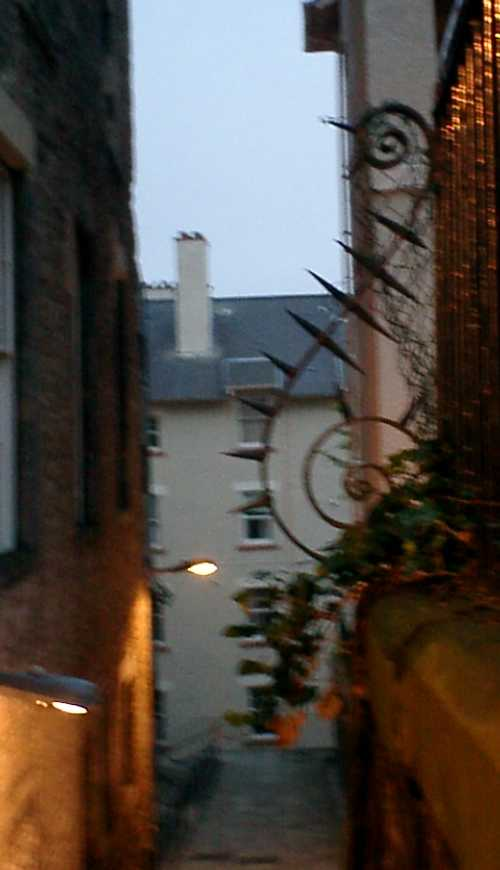
\includegraphics[width=1\hsize]{image200707/gurutitle.jpg}
\end{minipage}
\begin{minipage}{0.39\hsize}
 {\Huge #1
 }
\end{minipage}
\end{frame}
}

% 三択問題用
\newcounter{santakucounter}
\newcommand{\santaku}[5]{%
\addtocounter{santakucounter}{1}
\frame{\frametitle{問題\arabic{santakucounter}. #1}
%問題\arabic{santakucounter}. #1
\begin{minipage}[t]{0.8\hsize}
 \begin{itemize}
 \item
      \begin{minipage}{0.2\hsize}
      
\includegraphics[width=0.9\hsize]{image200703/janken-A.png}\end{minipage} 
       \begin{minipage}{0.6\hsize}
       A #2\end{minipage}\\
 \item
      \begin{minipage}{0.2\hsize}
      
\includegraphics[width=0.9\hsize]{image200703/janken-B.png}\end{minipage} 
       \begin{minipage}{0.6\hsize}
       B #3\end{minipage}\\
 \item
      \begin{minipage}{0.2\hsize}
      
\includegraphics[width=0.9\hsize]{image200703/janken-C.png}\end{minipage} 
       \begin{minipage}{0.6\hsize}
       C #4\end{minipage}\\
 \end{itemize}
\end{minipage}
}
\frame{\frametitle{問題\arabic{santakucounter}. #1}
%問題\arabic{santakucounter}. #1
\begin{minipage}[t]{0.8\hsize}
\begin{itemize}
 \item
      \begin{minipage}{0.2\hsize}
      
\includegraphics[width=0.9\hsize]{image200703/janken-A.png}\end{minipage} 
       \begin{minipage}{0.6\hsize}
       A #2\end{minipage}\\
 \item
      \begin{minipage}{0.2\hsize}
      
\includegraphics[width=0.9\hsize]{image200703/janken-B.png}\end{minipage} 
       \begin{minipage}{0.6\hsize}
       B #3\end{minipage}\\
 \item
      \begin{minipage}{0.2\hsize}
      
\includegraphics[width=0.9\hsize]{image200703/janken-C.png}\end{minipage} 
       \begin{minipage}{0.6\hsize}
       C #4\end{minipage}\\
\end{itemize}
\end{minipage}
\begin{minipage}[t]{0.15\hsize}
答えは:

\vspace{1cm}

  {\huge \hspace{1cm}#5}
  \hspace{-6cm}\includegraphics[width=4cm]{image200703/janken-#5.png}
 \end{minipage}}
}

\begin{document}
\frame{\titlepage{}}

\section{Intro}

\begin{frame}
 \frametitle{agenda}
\begin{minipage}[t]{0.45\hsize}
  \begin{itemize}
  \item Debconf7 紹介
	\begin{itemize}
	 \item 歴史
	 \item 会場
	 \item メンバー
	\end{itemize}
 \end{itemize}
\end{minipage} 
\begin{minipage}[t]{0.45\hsize}
 \begin{itemize}
  \item 討議内容
	\begin{itemize}
	 \item 組込み ARM EABI, Emdebian, Superh
	 \item i18n
	 \item 品質管理
	\end{itemize}  
  \item Q\&A
 \end{itemize}
\end{minipage}
\end{frame}

\emtext{Debconf7紹介}

\section{Debconf7 紹介}
\begin{frame}{歴史}
Debian Project の開発者をあつめて技術的な内容を討議する年次のカンファレンス
 \begin{tabular}{|c|c|c|r|}
 \hline
 年 & 名前 & 場所 & 参加人数 \\
 \hline
 2000 & debconf 0 &フランス ボルドー & \\
 2001 & debconf 1 &フランス ボルドー & \\
 2002 & debconf 2 &カナダ トロント & 90名 \\
 2003 & debconf 3 &ノルウェー オスロ & 140名 \\
 2004 & debconf 4 &ブラジル ポルトアレグレ &  150名 \\
 2005 & debconf 5 &フィンランド ヘルシンキ & 200名 \\
 2006 & debconf 6 &メキシコ オアスタペック & 300名 \\
 2007 & debconf 7 &スコットランド エジンバラ & 400名 \\
 2008 & debconf 8 &アルゼンチン マルデプラタ & ?名 \\
 \hline
 \end{tabular}
\end{frame}

\begin{frame}{会場 1/2}
\begin{minipage}{0.49\hsize}
 会場は昼の会場(Teviot)と夜の会場(廃教会)にわかれた。

  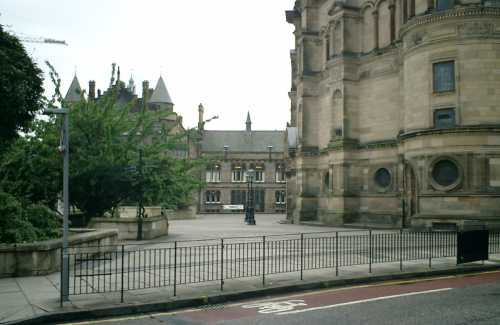
\includegraphics[width=1\hsize]{image200707/teviot.jpg}
\end{minipage}
\begin{minipage}{0.49\hsize}
  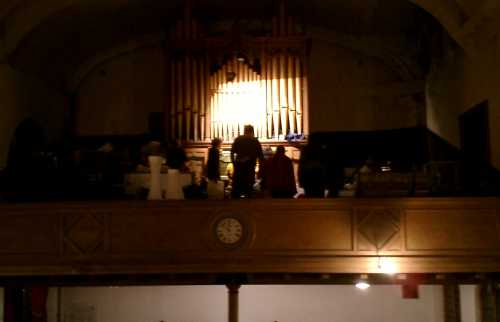
\includegraphics[width=1\hsize]{image200707/nightvenue1.jpg}\\
  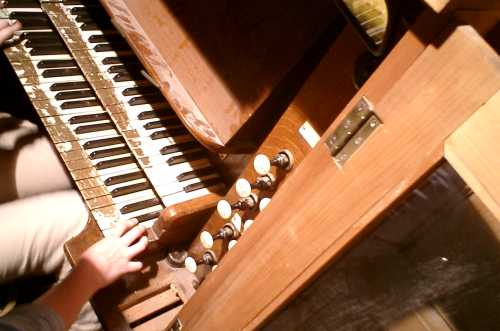
\includegraphics[width=1\hsize]{image200707/nightvenue2.jpg}
\end{minipage}
\end{frame}

\begin{frame}{会場 2/2}
\begin{minipage}{0.49\hsize}
  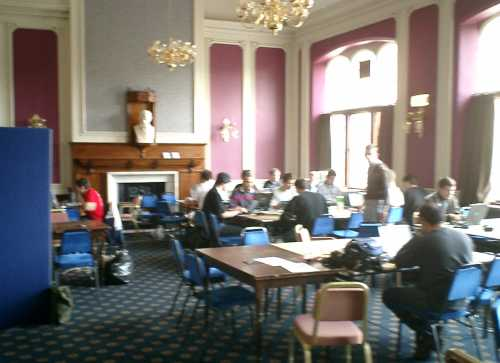
\includegraphics[width=1\hsize]{image200707/hacklab.jpg}\\
  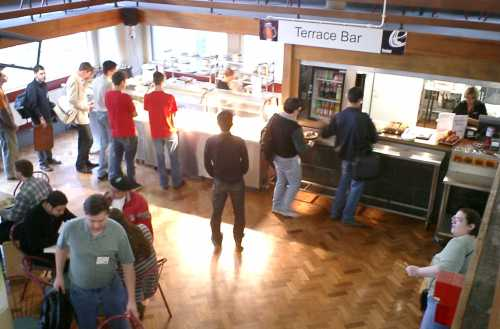
\includegraphics[width=1\hsize]{image200707/lunchplace.jpg}
\end{minipage}
\begin{minipage}{0.49\hsize}
  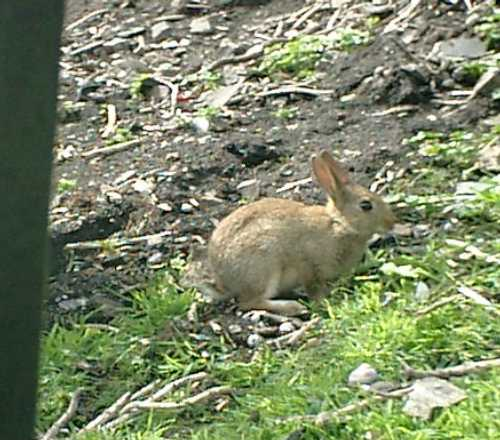
\includegraphics[width=1\hsize]{image200707/rabbit.jpg}\\
  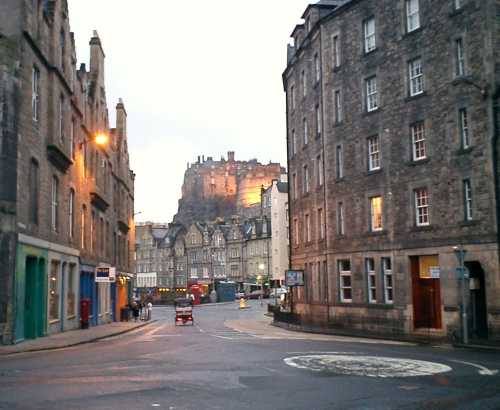
\includegraphics[width=1\hsize]{image200707/castle.jpg}
\end{minipage}
\end{frame}

\begin{frame}{アジェンダ 1/2}
  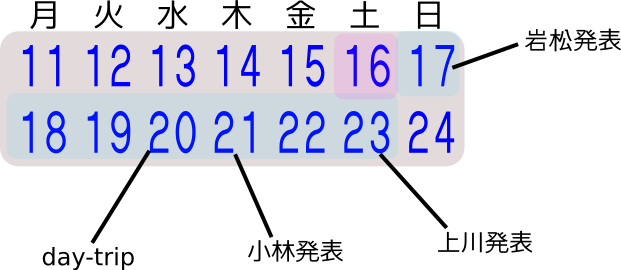
\includegraphics[width=1\hsize]{image200707/schedule.png}\\
発表内容:\\
岩松: superh 移植版について\\
小林: i18n関連\\
上川: pbuilder, cowbuilder, qemubuilder
\end{frame}

\begin{frame}{アジェンダ 2/2}
  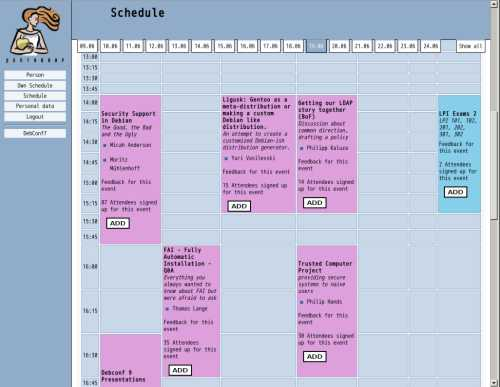
\includegraphics[height=0.6\vsize]{image200707/penta.png}\\
 スケジュールは pentabarf システムで管理、随時変更がかかる

 IRC チャンネルで IRC bot が開催が近くなると通知
\end{frame}

\begin{frame}{参加メンバー}
 2007年は日本からは岩松、矢吹、上川が参加

  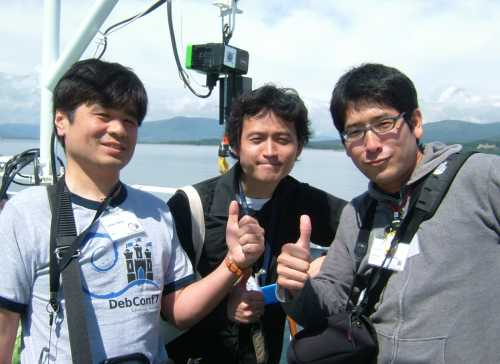
\includegraphics[width=1\hsize]{image200707/members.jpg}
\end{frame}

\begin{frame}{day-trip}
\begin{minipage}{0.5\hsize}
Bute 島への一日旅行

コンピュータに全く触れない一日をスケジュールの真ん中に準備することで長い
 会期をのりきる

新しいインスピレーションがうまれたり

新しいコミュニケーションができたり
\end{minipage}
\begin{minipage}{0.48\hsize}
  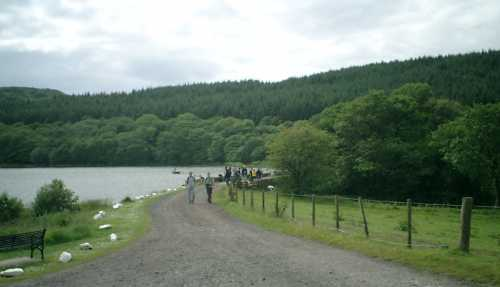
\includegraphics[width=1\hsize]{image200707/daytrip1.jpg}\\
  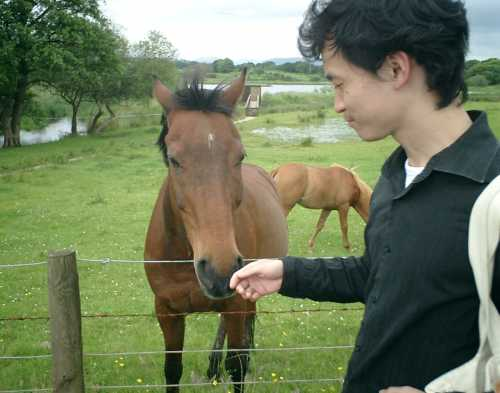
\includegraphics[width=1\hsize]{image200707/daytrip2.jpg}
\end{minipage}
\end{frame}

\emtext{討議内容}

\section{組込 関係の話題}
\begin{frame}
\frametitle{組込 関係の話題}
\begin{itemize}
\item Armel port
\item Emdebian
\item SuperH
\end{itemize}
\end{frame}

\section{Armel port}
\begin{frame}
\frametitle{Armel port} 
  \begin{minipage}{0.45\hsize}
    \begin{itemize}
      \item 発表者

	Wooky
    \end{itemize}
  \end{minipage}
  \begin{minipage}{0.45\hsize}
    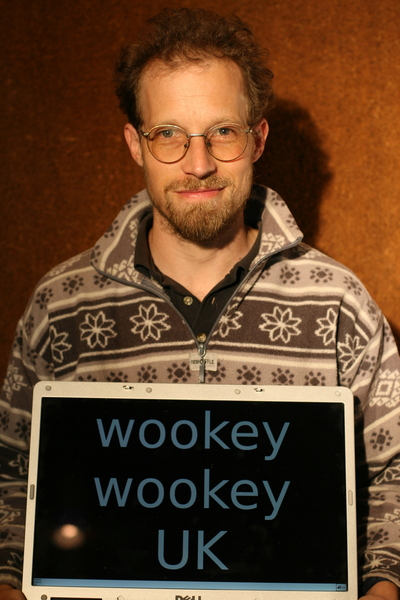
\includegraphics[width=4cm]{image200707/wookey.jpg}
  \end{minipage}

\end{frame}

\begin{frame}
\frametitle{Armelとは} 
\begin{itemize}
  \item Armel

     ARM への新しい ポーティング名 

  \item 二種類の ABI
    \begin{itemize}
	\item legacy ABI

	  従来の ABI
        \item ARM EABI

	  組込向けの ABI 
    \end{itemize}
\end{itemize}
\end{frame}

\begin{frame} 
\begin{itemize}
  \item legacy ABI
    \begin{itemize}
     
	\item FPU 命令コードの取扱い
	\item 例外による浮動小数点演算
    \end{itemize}

  \item EABI
    \begin{itemize}
	\item 動的な FPU を使った計算とソフトウェアによる計算
    \end{itemize}
\end{itemize}
  この2つに互換性はない
\end{frame}


\begin{frame}
\frametitle{現在の状況} 
\begin{itemize}
  \item binutils

	2.16.92 からサポート
  \item gcc
	
	gcc-4.1.1 からサポート
  \item glibc
	
	glibc-2.4 からサポート
  \item linux-kernel

	2.6.16 からサポート
  \item Debian packages

	現在、約10000パッケージをサポート
\end{itemize}
\end{frame}


\begin{frame}
\frametitle{今後の課題} 
\begin{itemize}
  \item 旧バイナリから新バイナリへの移行

	debtakeover\footnote{他のLinuxディストリからDebianに移行するための補助ツール} 
	を使うことによって、移行が容易になるはず。
 

\end{itemize}
\end{frame}


\section{Emdebian}
\begin{frame}
\frametitle{発表者} 
  \begin{minipage}{0.3\hsize}
    \begin{itemize}
      \item 発表者

	Wooky

        Neil Williams
    \end{itemize}
  \end{minipage}
  \begin{minipage}{0.6\hsize}
    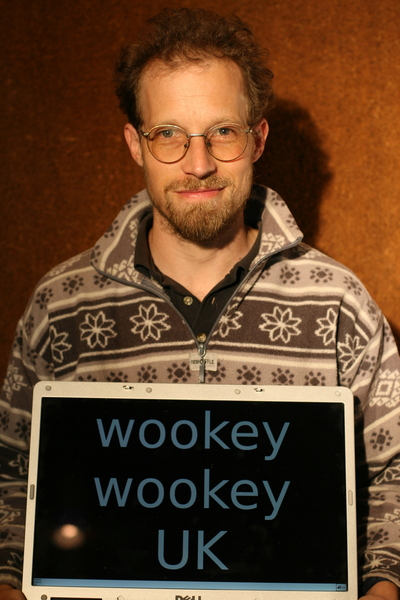
\includegraphics[width=4cm]{image200707/wookey.jpg}
    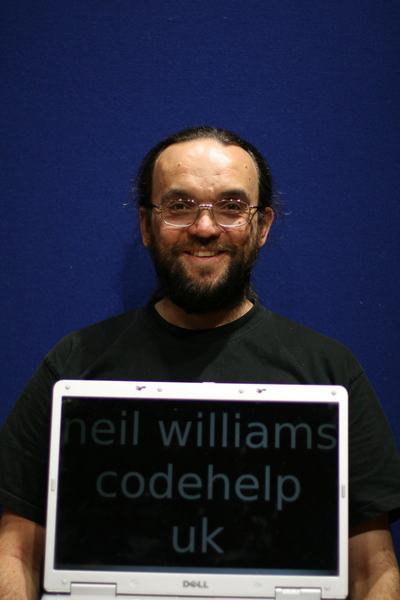
\includegraphics[width=4cm]{image200707/codehelp.jpg}  
  \end{minipage}

\end{frame}

\begin{frame} 
\frametitle{Emdebian}
  \begin{itemize}
    \item 2000 年から開始.
    \item Debian の組込向け プロジェクト
    \item 正式なサブプロジェクトのひとつ
    \item クロスコンパイルによるパッケージのサポート 
  \end{itemize}
\end{frame}

\begin{frame} 
\frametitle{いままで試してきたことについて}
  \begin{itemize}
    \item Debian は native コンパイル思考

	→ クロスコンパイルをサポートするように、パッケージにサポート修正

    \item Debian は パッケージサイズが大きく、デスクトップ思考
	
	→ パッケージを作成するときにドキュメントを外す仕組みを追加

    \item ソフトウェア毎に最適化する仕組み

    \item glibc 以外の C library を試用

    \item perl に頼らない Debian system の構築

	→ Essential から Perl package を外す
  \end{itemize}
\end{frame}


\begin{frame} 
\frametitle{現在のステータス}
  \begin{itemize}
    \item dpkg, apt, debhelper に cross 用のツールを追加
    \item cross 用のツールを用意

	\begin{itemize}
		\item dpkg-cross
		\item apt-cross
		\item emdebian-tools
		  %debuild → emdebuild
		  %dh_make → em_make
	\end{itemize}
    \item ドキュメント類を削除したパッケージを用意
    \item emdebian の changelog, patch を subversion で管理
    \item i386/ppc/amd64 用のクロスコンパイル環境の提供 
  \end{itemize}
\end{frame}


\begin{frame} 
\frametitle{解決すべき問題点など}
  \begin{itemize}
    \item configure のクロスコンパイル対応

	configure 実行するときに --host, --target を指定していないものが多い

    \item configure のドキュメント対応

	-nodocs, -nocheck に対応していない configure が多い

    \item テストプログラム

	コンパイル途中で動作するテストプログラムを実行しないで済む仕組みが
	必要 
  \end{itemize}
\end{frame}



\begin{frame} 
\frametitle{今後の予定}
  \begin{itemize}
    \item ツールチェイン自動アップデート
    \item GPE for ARM
    \item emdebuild
    \item empdebuild
    \item configure キャッシュファイルのサポート 
  \end{itemize}
\end{frame}


\begin{frame} 
\frametitle{Emdebian BOF}
  \begin{itemize}
    \item uClibc サポートの議論
	\begin{itemize}
	  \item バイナリ非互換
	  \item メンテナンス性、サーバー容量の問題
	\end{itemize}
    \item Busybox サポートの議論
	\begin{itemize}
	  \item GPE が 使用
	  \item busybox 上でのパッケージサポート
	\end{itemize}
  \end{itemize}
\end{frame}


\section{Debian for SuperH}
\begin{frame}
\frametitle{Debian for SuperH} 
  \begin{minipage}{0.4\hsize}
    \begin{itemize}
      \item 発表者

	Nobuhiro Iwamatsu
    \end{itemize}
  \end{minipage}
  \begin{minipage}{0.4\hsize}
    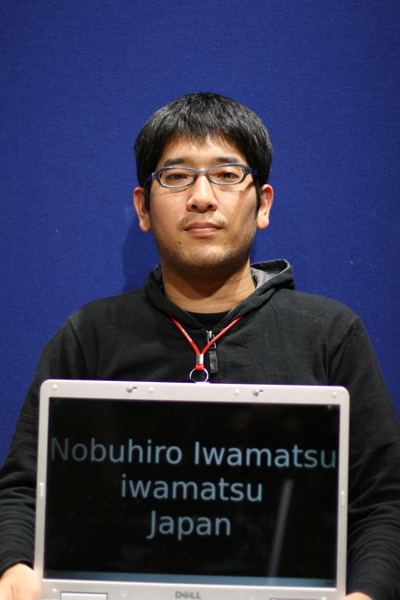
\includegraphics[width=4cm]{image200707/iwamatsu.jpg}  
  \end{minipage}
\end{frame}


\begin{frame} 
\frametitle{今までの移植の歴史}
  \begin{itemize}
    \item 自分が行うまでに2回移植が行われた
    \item しかし、全て失敗
    \item 世界を巻き込んでやらないといけない

	世界の興味ある人を募集中。 
  \end{itemize}
\end{frame}


\begin{frame} 
\frametitle{ポーティングポリシー}
  \begin{itemize}
    \item サポートアーキテクチャ

	SH4 / little

    \item SH3 : FPU / Calling convention / Cache   
    \item Big Endian
	
  \end{itemize}
\end{frame}


\begin{frame} 
\frametitle{現在の状況}
  \begin{itemize}
    \item Maling list
    \item Buildd 動作中   
    \item Build-essential
    \item 2000パッケージビルド
  \end{itemize}
\end{frame}

\begin{frame} 
\frametitle{TODO}
  \begin{itemize}
    \item buildd / アーキテクチャ メンテナンスチーム
    \item SH 特有の問題を解決   
    \item Buildd.net への登録
  \end{itemize}
\end{frame}


\begin{frame} 
\frametitle{現在入手可能な SH デバイス紹介}
  \begin{itemize}
    \item ULS-5P
    \item T-SH7706-LAN   
    \item L-BOX
    \item PX-EH16L
  \end{itemize}
\end{frame}

\begin{frame} 
\frametitle{議論}
  \begin{itemize}
    \item SH4A コアなどの対応
    \item キャッシュ問題の回避方法
    \item マシンの入手の問題
  \end{itemize}
\end{frame}

\section{i18n 関係の話題}

\begin{frame}
\frametitle{i18n 関係の話題} 
Debconf7 で行われた i18n (internationalization) のセッション
  \begin{itemize}
     \item i18n work session
     \item Quality assurance activities for localization    
  \end{itemize}
\end{frame}


\begin{frame}
\frametitle{i18n work session} 
  \begin{minipage}{0.4\hsize}
    \begin{itemize}
      \item 発表者

	Christian Perrier
    \end{itemize}
  \end{minipage}
  \begin{minipage}{0.4\hsize}
    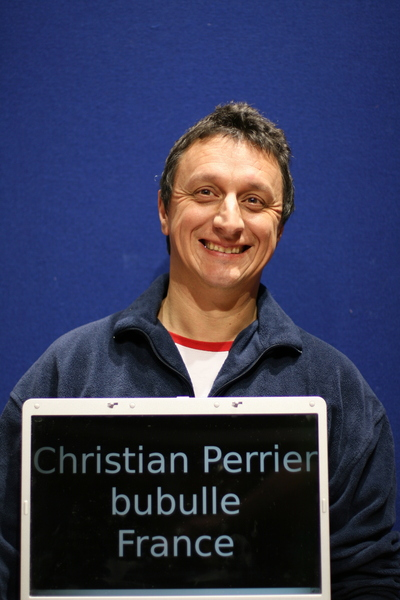
\includegraphics[width=4cm]{image200707/bubulle.jpg}  
  \end{minipage}
\end{frame}

\begin{frame}
\frametitle{i18n work session} 
期間中に8回のセッションが行われた.

  \begin{itemize}
     \item Launch session
     \item Lenny i18n release goals
     \item Pootle session
     \item DDTP, DDTSS, discussion about DDTP import to Pootle
     \item i18n  translation licensing, website, documentation
     \item i18n No content yet..:-)
     \item "tdebs", dpkg/apt, classes of files
     \item Conclusion session    
    
  \end{itemize}
\end{frame}

\begin{frame}
\frametitle{Quality assurance activities for localization} 
  \begin{minipage}{0.4\hsize}
    \begin{itemize}
      \item 発表者

	\sout{Noritada Kobayashi}

        代打 Junichi Uekawa
    \end{itemize}
  \end{minipage}
  \begin{minipage}{0.4\hsize}
    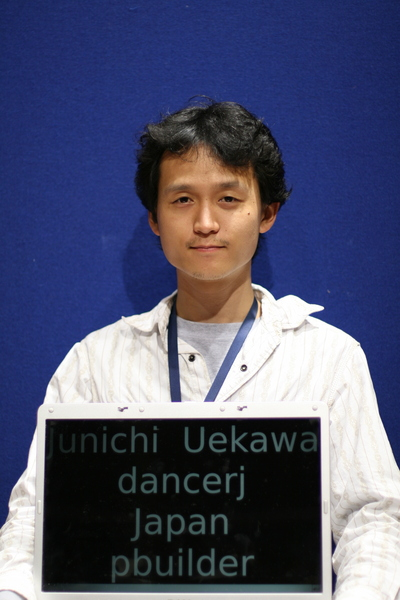
\includegraphics[width=4cm]{image200707/dancerj.jpg}  
  \end{minipage}
\end{frame}


\begin{frame}
\frametitle{セッション内容}

  どのようなツールを使って翻訳を行っているのか.
  \begin{itemize}
    \item pootle

	翻訳向けポータルサイトツール
	\url{i18n.debian.net:8080}
    \item robot

	現在、Debian 翻訳チームが使っているツール
	\url{i18n.debian.net/debian-l10n}\\
    \item 翻訳ツール
	\begin{itemize}
	  \item emacs/vi po-mode
          \item poedit
        \end{itemize}

    \item 翻訳補助ツール
	\begin{itemize}
	   \item kbabel / vi spell check など 
	   \item pootel でも可能
	\end{itemize}

    \item 現在のワークフローや情報

	\url{http://i18n.debian.net/wiki}
  \end{itemize}
\end{frame}


\section{品質管理 関係の話題}
\begin{frame} 
\frametitle{品質管理 関係の話題}

  \begin{itemize}
    \item Proactive Bug Discovery
    \item Maintaining Packages With Git
    \item WTFM, again: Write The Fine Manual page
  \end{itemize}
%Automated Testing of Debian Packages: Status Update
%bugs.debian.org and debbugs
%Debian Documentation Project: current status and future
%Debtags is ready
%Forking Debian every day
\end{frame}



\begin{frame} 
\frametitle{WTFM, again: Write The Fine Manual page}
  \begin{minipage}{0.4\hsize}
    \begin{itemize}
      \item 発表者

	W. Borgert
    \end{itemize}
  \end{minipage}
  \begin{minipage}{0.4\hsize}
    No Photo  
  \end{minipage}
\end{frame}

\begin{frame} 
\frametitle{WTFM, again: Write The Fine Manual page}
  いかにして、品質のよい man page を作成するか.

  \begin{itemize}
    \item Debian で頒布されているプログラムにはマニュアルが必要
    \item nroff 形式の man が多いが時代遅れ

	あらゆるフォーマットに対応できる形式が望ましい
    \item docbok-xml を使うとよい
	
	Gnome, KDE, Linux などで採用
    \item マニュアルがソースに含まれている場合もあるが、チェックが必要
  \end{itemize}	
\end{frame}

\begin{frame} 
\frametitle{Proactive Bug Discovery}
  \begin{minipage}{0.4\hsize}
    \begin{itemize}
      \item 発表者

	Sam Hocevar / Debian Project Leader
    \end{itemize}
  \end{minipage}
  \begin{minipage}{0.4\hsize}
    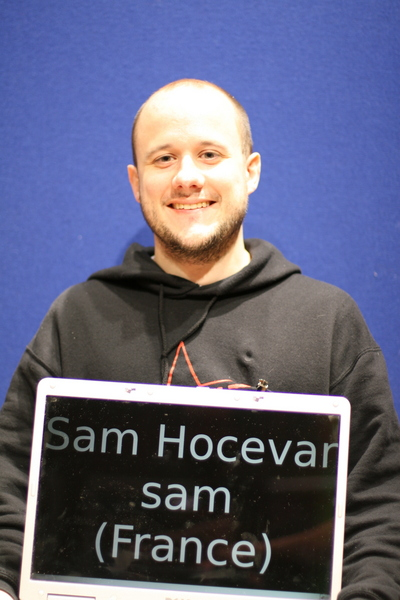
\includegraphics[width=4cm]{image200707/sam.jpg}
  \end{minipage}
\end{frame}

\begin{frame} 
\frametitle{Proactive Bug Discovery}
  パッケージの不具合を見つけるには

  \begin{itemize}
    \item ソースコードから見つける
	\begin{itemize}
	  \item google code search
	  \item rats, pscan, jlint, pychecker
	\end{itemize}

    \item コンパイル時に -Wall をつけよう
    \item makewrap の活用
	
	LD\_PRELOAD=makewrap.so debian/rules
	
    \item build log を参照

	http://buildd.debian.org

  \end{itemize}	
\end{frame}


\begin{frame} 
\frametitle{Proactive Bug Discovery}
  バイナリパッケージから不具合を見つける

  \begin{itemize}
    \item Debian Policy によるチェック
	
	linda / lintian
	
    \item インストール/アンインストールチェック

	piuparts

    \item Fuzzing の活用
	
	zzuf パッケージを使ったテスト方法

    \item GUI アプリケーション のデバッグ
	
	xvfb の活用

    \item test suite の活用

  \end{itemize}	
\end{frame}


\begin{frame} 
\frametitle{Maintaining Packages With Git}
  \begin{minipage}{0.4\hsize}
    \begin{itemize}
      \item 発表者

	David Nusinow
    \end{itemize}
  \end{minipage}
  \begin{minipage}{0.4\hsize}
    no photo
  \end{minipage}
\end{frame}


\begin{frame} 
\frametitle{Maintaining Packages With Git}
  git, git-buildpackage を使って、debian package を管理する方法
	
  \begin{itemize}
    \item X strikeforce は gitを使っている
    \item patch 管理 は quilt を使う
    \item git を使うだけで時間の節約になる
    
	各種ツールがはやい. branch が楽.

    \item svn ではコミットに制限があるが git にはない

	どこでもコミット.

    \item git-xxx

	他の SCM で管理しているアップストリームを git で管理するのに楽

	
  \end{itemize}
\end{frame}


\begin{frame} 
\frametitle{Maintaining Packages With Git}
  git, git-buildpackage を使って、debian package を管理する方法
	
  \begin{itemize}
    \item debcommit
	debian/changelog を各 SCM のコミットメッセージとして扱ってくれるツール

    \item 問題
      \begin{itemize}
	 \item git-buildpackage は
	       アップストリームが git を使っている場合に、うまく動作しない
	 \item git の Windows ネイティブ版が普及していない\footnote{
	       cygwin 版、mingw 版はある }
         \item git ではディレクトリ毎にチェックアウトできない\footnote{submodule
	       機能実装中}
      \end{itemize}
  \end{itemize}
 
\end{frame}


\section{Debconf7 の情報}
\begin{frame} 
\frametitle{Debconf7の情報 }
\begin{itemize}
    \item \url{http://debconf7.debconf.org}
    \item \url{http://wiki.debconf.org/wiki/DebConf7}
  \end{itemize}
\end{frame}

\section{次の Debconf}
\begin{frame} 
\frametitle{次の Debconf }
\begin{center}

\includegraphics[width=10cm]{image200707/debconf8.png}  
 \end{center}  
\begin{itemize}
    \item アルゼンチン
    \item 8月 (開催地は冬です)
  \end{itemize}
\end{frame}
\end{document}
